\documentclass{article}
\usepackage{LaTeX-Submodule/template}

\usepackage{chngcntr} % Reset counter within sections
\usepackage{circuitikz}
\DeclareSIUnit{\nothing}{\relax}

\counterwithin*{equation}{section}
\counterwithin*{equation}{subsection}
\counterwithin*{remark}{subsection}

\pagestyle{fancy}
\setlength\headheight{24pt}
\setlength\parindent{0pt}

\lhead{\className}
\rhead{\leftmark}
\cfoot{\thepage}

\newcommand{\className}{Foundations of Electrical Engineering}
\newcommand{\classTime}{Semester 2, 2021}
\newcommand{\classInstructorName}{Dr Jasmin Martin}

\usepackage[
    type={CC},
    modifier={by-nc-sa},
    version={4.0},
    imagewidth={5em},
    hyphenation={raggedright}
]{doclicense}

\date{}

\begin{document}

\begin{titlepage}
    \vspace*{\fill}
    \begin{center}
        \LARGE{\textbf{\className}}
        \texorpdfstring{\\}{ }
        \texorpdfstring{\vspace{0.1in}}{ }
        \normalsize{\classTime}
        \texorpdfstring{\\}{ }
        \texorpdfstring{\vspace{0.1in}}{ }
        \normalsize\textit{\classInstructorName}
        \texorpdfstring{\\}{ }
        \texorpdfstring{\vspace{0.2in}}{ }
        \textsc{Tarang Janawalkar}
    \end{center}
    \vspace*{\fill}
    \doclicenseThis
    \thispagestyle{empty}
\end{titlepage}
\newpage

\tableofcontents
\newpage

\section{Electrical Circuits}
\subsection{SI Prefixes}
\begin{table}[H]
    \centering
    \begin{minipage}[H]{0.48\linewidth}
        \centering
        \begin{tabular}{c c c}
            \toprule
            \textbf{Factor} & \textbf{Name} & \textbf{Symbol}       \\
            \midrule
            $10^{24}$       & yotta         & \unit{\yotta\nothing} \\
            $10^{21}$       & zetta         & \unit{\zetta\nothing} \\
            $10^{18}$       & exa           & \unit{\exa\nothing}   \\
            $10^{15}$       & peta          & \unit{\peta\nothing}  \\
            $10^{12}$       & tera          & \unit{\tera\nothing}  \\
            $10^{9}$        & giga          & \unit{\giga\nothing}  \\
            $10^{6}$        & mega          & \unit{\mega\nothing}  \\
            $10^{3}$        & kilo          & \unit{\kilo\nothing}  \\
            \bottomrule
        \end{tabular}
    \end{minipage}
    \begin{minipage}[H]{0.48\linewidth}
        \centering
        \begin{tabular}{c c c}
            \toprule
            \textbf{Factor} & \textbf{Name} & \textbf{Symbol}       \\
            \midrule
            $10^{-3}$       & milli         & \unit{\milli\nothing} \\
            $10^{-6}$       & micro         & \unit{\micro\nothing} \\
            $10^{-9}$       & nano          & \unit{\nano\nothing}  \\
            $10^{-12}$      & pico          & \unit{\pico\nothing}  \\
            $10^{-15}$      & femto         & \unit{\femto\nothing} \\
            $10^{-18}$      & atto          & \unit{\atto\nothing}  \\
            $10^{-21}$      & zepto         & \unit{\zepto\nothing} \\
            $10^{-24}$      & yocto         & \unit{\yocto\nothing} \\
            \bottomrule
        \end{tabular}
    \end{minipage}
    \caption{SI prefixes.}
    % \label{}
\end{table}
\subsection{Fundamental Quantities}
\begingroup
\renewcommand{\arraystretch}{1.5}
\begin{table}[H]
    \centering
    \begin{tabular}{c | >{\centering}p{0.5\textwidth} | c | c}
        \toprule
        \textbf{Name} & \textbf{Definition}                                                                                                      & \textbf{Symbol}           & \textbf{Unit} \\
        \midrule
        Charge        & Electric charge is a fundamental property of matter that governs how particles are affected by an electromagnetic field.
                      & $q$                                                                                                                      & Coulomb (\unit{\coulomb})                 \\
        \hline
        Current       & $\displaystyle i = \dv{q}{t}\iff\SI{1}{\ampere} = \SI{1}{\coulomb\per\s}$
                      & $i$                                                                                                                      & Ampere (\unit{\ampere})                   \\
        \hline
        Voltage       & $\displaystyle v = \dv{w}{q}\iff\SI{1}{\volt} = \SI{1}{\joule\per\coulomb}$
                      & $v$                                                                                                                      & Volt (\unit{\volt})                       \\
        \hline
        Power         & $\displaystyle p = \dv{w}{t}\iff\SI{1}{\watt} = \SI{1}{\joule\per\s}$
                      & $p$                                                                                                                      & Watt (\unit{\watt})                       \\
        \bottomrule
    \end{tabular}
    \caption{Fundamental quantities in electrical circuits.}
\end{table}
\endgroup
\begin{description}
    \item[Charge in an electron.] $q = \SI{1.6022e-19}{\coulomb}$.
    \item[Electric Power.] $\displaystyle p = \dv{w}{t} = vi$.
\end{description}
\subsection{Passive Sign Convention}
\begin{figure}[H]
    \centering
    \begin{minipage}[H]{0.48\textwidth}
        \centering
        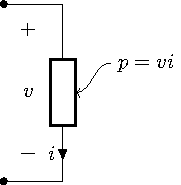
\includegraphics[height = 4cm, keepaspectratio = true]{passive_component}
        \caption{Energy dissipated.}
    \end{minipage}\hfill
    \begin{minipage}[H]{0.48\textwidth}
        \centering
        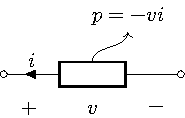
\includegraphics[height = 4cm, keepaspectratio = true]{active_component}
        \caption{Energy produced.}
    \end{minipage}
\end{figure}
\begin{theorem}[Power Balance]
    \begin{equation*}
        p_{\mathrm{net}} = 0
    \end{equation*}
\end{theorem}
\begin{theorem}[Energy]
    \begin{equation*}
        w\left( \tau \right) = \int_0^\tau p\left( t \right) \dd{t}
    \end{equation*}
\end{theorem}
\subsection{Circuits and Sources}
\begin{definition}[Circuits]
    A circuit is a mathematical model that approximates a real system. It is built from ideal circuit elements connected by ideal wires.
\end{definition}
\begin{definition}[Voltage Source]
    Produces or dissipates power at a specified voltage with whatever current is required.
\end{definition}
\begin{figure}[H]
    \centering
    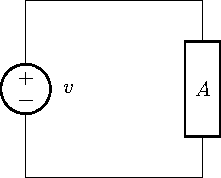
\includegraphics[height = 4cm, keepaspectratio = true]{voltage_source}
    \caption{Voltage source -- $v$ is specified, $i$ varies depending on circuit element $A$.}
\end{figure}
\begin{definition}[Current Source]
    Produces or dissipates power at a specified current with whatever voltage is required.
\end{definition}
\begin{figure}[H]
    \centering
    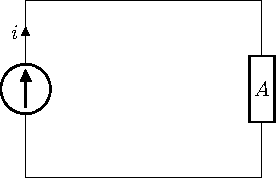
\includegraphics[height = 4cm, keepaspectratio = true]{current_source}
    \caption{Current source -- $i$ is specified, $v$ varies depending on circuit element $A$.}
\end{figure}
\subsection{Resistors}
\begin{definition}[Resistor]
    Resistors dissipate power, and the voltage across both terminals is proportional to the current.
\end{definition}
\begin{figure}[H]
    \centering
    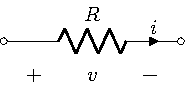
\includegraphics[height = 3cm, keepaspectratio = true]{resistor}
    \caption{Resistor circuit symbol.}
\end{figure}
\begin{theorem}[Voltage through a resistor]
    \begin{equation*}
        v = iR
    \end{equation*}
\end{theorem}
\begin{corollary}[Power dissipated by a resistor]
    \begin{equation*}
        p = vi = i^2 R = \frac{v^2}{R}
    \end{equation*}
\end{corollary}
\newpage
\section{Simple Resistive Circuits}
\subsection{Ignored Physics}
\begin{enumerate}
    \item Electrical effects occur instantaneously, so there is no time delay along the wires.
    \item The net charge on every component is zero. Charge is never lost or gained.
    \item There is no magnetic coupling between the components.
\end{enumerate}
\subsection{Kirchhoff's Laws}
\begin{theorem}[Kirchhoff's Current Law (KCL)]
    The sum of all currents into a node equals zero.
    \begin{equation*}
        \sum i_{\mathrm{node}} = 0
    \end{equation*}
\end{theorem}
\begin{theorem}[Kirchhoff's Voltage Law (KVL)]
    The sum of all voltages around a loop equals zero.
    \begin{equation*}
        \sum v_{\mathrm{loop}} = 0
    \end{equation*}
\end{theorem}
\subsection{Series and Parallel Circuits}
\begin{definition}
    Elements connected end-to-end are in series. If both ends of an element are connected directly to another element, the two elements are in parallel.
\end{definition}
\begin{table}[H]
    \centering
    \begin{tabular}{c | c c}
        \toprule
        \textbf{Element} & \textbf{Series}                                                         & \textbf{Parallel}                                                       \\
        \midrule
        Current Source   & $\displaystyle i_{\mathrm{eq}} = i_{k\geq1}$                            & $i_{\mathrm{eq}} = \displaystyle \sum_{k\geq1} i_k$                     \\
        Voltage Source   & $\displaystyle v_{\mathrm{eq}} = \sum_{k\geq1} v_k$                     & $\displaystyle v_{\mathrm{eq}} = v_{k\geq1}$                            \\
        Resistor         & $\displaystyle R_{\mathrm{eq}} = \sum_{k\geq1} R_k$                     & $\displaystyle \frac{1}{R_{\mathrm{eq}}} = \sum_{k\geq1} \frac{1}{R_k}$ \\
        Inductor         & $\displaystyle L_{\mathrm{eq}} = \sum_{k\geq1} L_k$                     & $\displaystyle \frac{1}{L_{\mathrm{eq}}} = \sum_{k\geq1} \frac{1}{L_k}$ \\
        Capacitor        & $\displaystyle \frac{1}{C_{\mathrm{eq}}} = \sum_{k\geq1} \frac{1}{C_k}$ & $\displaystyle C_{\mathrm{eq}} = \sum_{k\geq1} C_k$                     \\
        \bottomrule
    \end{tabular}
    \caption{Equivalent values for various components connected in series and parallel.}
\end{table}
These equations can be used to simplify a complex circuit.
\subsection{Voltage and Current Dividers}
\begin{definition}[Voltage Divider]
    A voltage divider is a circuit that divides a voltage in the proportion of the series resistances.
\end{definition}
\begin{figure}[H]
    \centering
    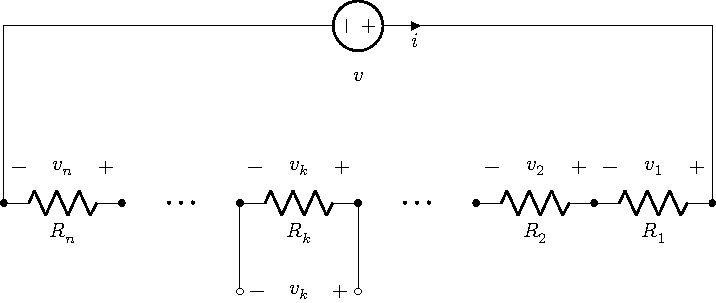
\includegraphics[height = 4cm, keepaspectratio = true]{voltage_divider}
    \caption{Voltage divider circuit.}
\end{figure}
\begin{theorem}[Voltage Divider]
    \begin{equation*}
        v_k = v \frac{R_k}{R_{\mathrm{eq}}}
    \end{equation*}
\end{theorem}
\begin{proof}
    The current through any resistor is
    \begin{equation*}
        i = \frac{v}{R_{\mathrm{eq}}}.
    \end{equation*}
    Therefore the voltage drop in any resistor is
    \begin{align*}
        v_k & = i R_k                          \\
        v_k & = \frac{v}{R_{\mathrm{eq}}} R_k.
    \end{align*}
\end{proof}
\begin{definition}[Current Divider]
    A voltage divider is a circuit that divides a voltage in the proportion of the series resistances.
\end{definition}
\begin{figure}[H]
    \centering
    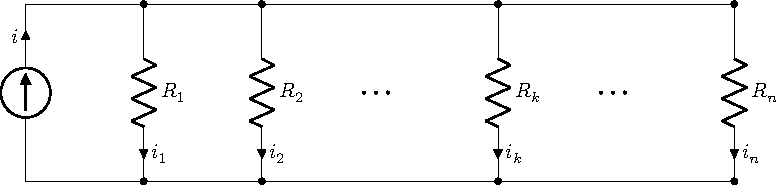
\includegraphics[height = 3cm, keepaspectratio = true]{current_divider}
    \caption{Current divider circuit.}
\end{figure}
\begin{theorem}[Current Divider]
    \begin{equation*}
        i_k = i \frac{R_{\mathrm{eq}}}{R_k}
    \end{equation*}
\end{theorem}
\begin{proof}
    Using KCL we have
    \begin{align*}
        i & = \sum_{k\geq1} i_k           \\
        i & = \sum_{k\geq1} \frac{v}{R_k} \\
        i & = \frac{v}{R_{\mathrm{eq}}}.
    \end{align*}
    Solving for $v$ gives
    \begin{align*}
        v & = i R_{\mathrm{eq}}.
    \end{align*}
    Hence the current through any resistor in parallel is given by
    \begin{align*}
        i_k = \frac{v}{R_k} = \frac{iR_{\mathrm{eq}}}{R_k}.
    \end{align*}
\end{proof}
\newpage
\section{Diodes}
\begin{definition}[Diode]
    A diode is a semiconductor component in which current flows only in one direction. A diode requires a voltage to start the flow of current in the forward direction.
    The forward voltage is commonly \SI{0.7}{\volt}.
\end{definition}
\begin{figure}[H]
    \centering
    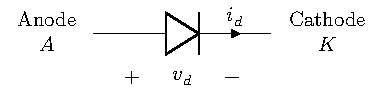
\includegraphics[height = 3cm, keepaspectratio = true]{diode}
    \caption{Diode circuit symbol.}
\end{figure}
\subsection{VI Characteristic}
The Voltage-Current characteristic of linear circuit elements can be plotted as shown below.
\begin{figure}[H]
    \centering
    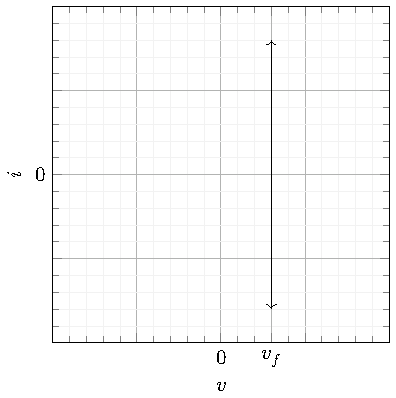
\includegraphics[height = 5cm, keepaspectratio = true]{vi_characteristic_voltage_source}
    \caption{VI characteristic for a voltage source.}
\end{figure}
\begin{figure}[H]
    \centering
    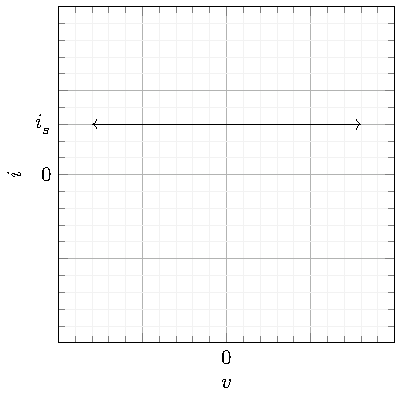
\includegraphics[height = 5cm, keepaspectratio = true]{vi_characteristic_current_source}
    \caption{VI characteristic for a current source.}
\end{figure}
\begin{figure}[H]
    \centering
    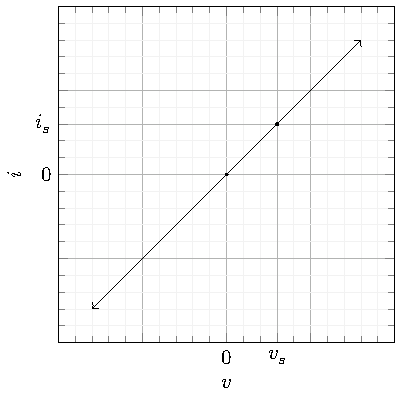
\includegraphics[height = 5cm, keepaspectratio = true]{vi_characteristic_resistor}
    \caption{VI characteristic for a resistor.}
\end{figure}
\subsection{VI Characteristic for Diodes}
A diode has a non-linear characteristic curve, hence it is often simplified.
\begin{figure}[H]
    \centering
    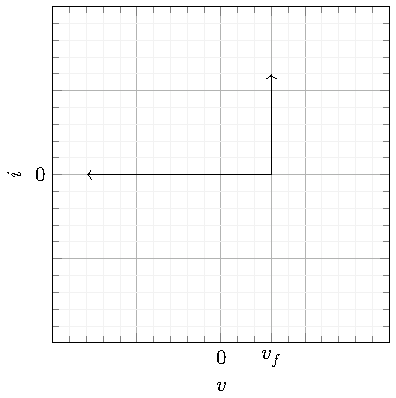
\includegraphics[height = 5cm, keepaspectratio = true]{vi_characteristic_diode}
    \caption{VI characteristic for a diode.}
\end{figure}
\begin{theorem}[Shockley's Diode Equation]
    A diode can be better modelled using Shockley's equation.
    \begin{equation*}
        i = I_S \exp{\left( \frac{v}{0.026} \right)}
    \end{equation*}
    where $I_S$ is the saturation current and $0.026$ is the thermal voltage.
\end{theorem}
\subsection{Operating Points and Load Lines}
\begin{definition}[Operating Point]
    The operating point for two elements can be found by determining the intersection
    of the two VI characteristic curves.
\end{definition}
\begin{definition}[Load Lines]
    If a circuit contains three or more elements including a diode, the VI characteristic curve
    is found around the diode. This curve is called a load line.
\end{definition}
\subsection{Operating Point of Non-Linear Component}
Given the following circuit with a non-linear component
\begin{figure}[H]
    \centering
    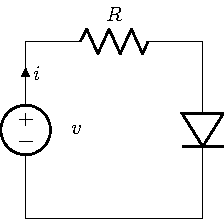
\includegraphics[height = 4cm, keepaspectratio = true]{non_linear_component}
    \caption{Circuit with non-linear element.}
\end{figure}
the load line is given by the equation
\begin{equation*}
    i(v) = -\frac{i_{sc}}{v_{oc}} + i_{sc}
\end{equation*}
where the short circuit current is the current through the non-linear component, and the open circuit voltage is the voltage across the
open circuit nodes of the component.
\begin{figure}[H]
    \centering
    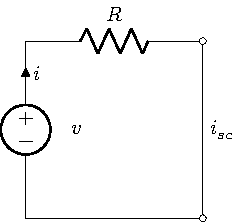
\includegraphics[height = 4cm, keepaspectratio = true]{non_linear_short_circuit_current}
    \caption{Circuit for short circuit current.}
\end{figure}
\begin{figure}[H]
    \centering
    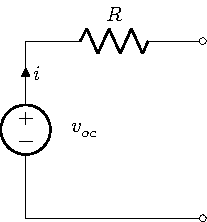
\includegraphics[height = 4cm, keepaspectratio = true]{non_linear_open_circuit_voltage}
    \caption{Circuit for open circuit voltage.}
\end{figure}
\newpage
\section{Mesh Analysis}
\begin{definition}[Node]
    A point where two or more circuit elements join.
\end{definition}
\begin{definition}[Essential Node]
    A point where three or more circuit elements join.
\end{definition}
\begin{definition}[Loop]
    A path with the same start and end node.
\end{definition}
\begin{definition}[Mesh]
    A loop that does not enclose any other loops.
\end{definition}
\subsection{Mesh Analysis Steps}
\begin{enumerate}
    \item Label the unknown mesh currents.
    \item Find the voltage across each of the circuit elements in terms of mesh currents.
    \item Use KVL around each mesh to create simultaneous equations.
    \item Solve simultaneous equations for mesh currents.
\end{enumerate}
\subsection{Mesh Analysis with Current Sources}
If the current source is in a single mesh, then treat the mesh current as known and solve as before.

If the current source is between two meshes, then we must use a supermesh.
\begin{definition}[Supermesh]
    A supermesh is a special mesh that surrounds the current source.
\end{definition}
\begin{enumerate}
    \item Label meshes and identify the supermesh.
    \item Write KCL equation for the current source.
    \item Write the supermesh equation.
    \item Use KVL around the supermesh.
\end{enumerate}
\newpage
\section{Source Transformations}
Real sources often have many limitations in terms of voltage and current delivery.
The most commonly modelled and most useful for linear circuit theory is some form of
resistance associated with the source.
\subsection{Thévenin Equivalent Circuit}
\begin{definition}
    The Thévenin equivalent circuit is a voltage source with a series resistance.
    \begin{figure}[H]
        \centering
        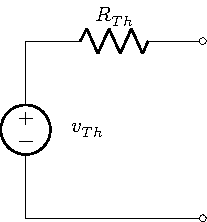
\includegraphics[height = 4cm, keepaspectratio = true]{thevenin_equivalent}
        \caption{Thévenin equivalent circuit.}
        % \label{}
    \end{figure}
    This circuit has the following properties:
    \begin{description}
        \item[Open circuit voltage.] $v_{oc} = v_{Th}$
        \item[Short circuit current.] $i_{sc} = \frac{v_{Th}}{R_{Th}}$
    \end{description}
\end{definition}
\subsection{Norton Equivalent Circuit}
\begin{definition}
    Similar to the Thévenin equivalent model, we can use a current source with
    a resistor in parallel to model the same circuit.
    \begin{figure}[H]
        \centering
        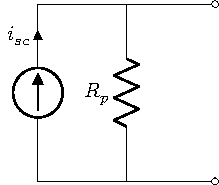
\includegraphics[height = 4cm, keepaspectratio = true]{norton_equivalent}
        \caption{Norton equivalent circuit.}
        % \label{}
    \end{figure}
    This circuit has the following properties:
    \begin{description}
        \item[Open circuit voltage.] $v_{oc} = i_{sc}R_{p}$
        \item[Short circuit current.] $i_{sc} = i_{sc}$
    \end{description}
\end{definition}
\subsection{Source Transformations}
A source transformation is the process of simplifying a circuit by transforming
voltage sources into current sources, and vice versa, using Thévenin's Theorem and Norton's
Theorem.
\begin{theorem}
    Thévenin and Norton equivalent circuits have the following relationship
    \begin{equation*}
        R_{Th} = R_{p}.
    \end{equation*}
\end{theorem}
\subsection{Superposition}
\begin{theorem}[Thévenin's Theorem]
    Any linear circuit can be replaced by a voltage source and a resistance in series.
\end{theorem}
\begin{theorem}[Norton's Theorem]
    Any linear circuit can be replaced by a current source and a resistance in parallel.
\end{theorem}
\begin{definition}[Turning Sources ``off'']
    Turning a source ``off'' means to set its value to 0.
    \begin{description}
        \item[For a voltage source:] $v = \SI{0}{\volt}$, hence we can treat it as a short circuit.
        \item[For a current source:] $i = \SI{0}{\ampere}$, hence we can treat it as an open circuit.
    \end{description}
\end{definition}
\subsubsection{Equivalent Sources}
To determine the equivalent voltage or current source between two nodes, we must
turn on each source in the circuit one by one, and calculate the voltage or current
between those nodes.
The equivalent voltage or current is equal to the sum of contributions from each source.
\subsubsection{Equivalent Resistance}
The equivalent resistance is determined by turning off all sources and calculating the
equivalent resistance between the two nodes.
\subsection{Maximum Power Transfer}
In the circuit shown below, the maximum power transfer to the load is given by
\begin{equation*}
    P_L = \frac{v_{Th}^2}{4R_L}
\end{equation*}
where $R_L = R_{Th}$.
\begin{figure}[H]
    \centering
    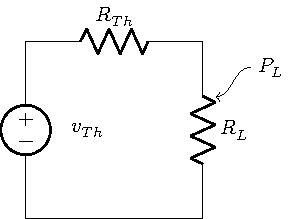
\includegraphics[height = 4cm, keepaspectratio = true]{max_power_transfer}
    \caption{Power transfer in a Thévenin model.}
\end{figure}
\newpage
\section{Inductors and Capacitors}
\subsection{Capacitors}
\begin{definition}
    Capacitors store electrical energy as a voltage. The ratio of voltage
    to charge across a capacitor is its capacitance, measured in Farads (\si{\farad}).
    \begin{equation*}
        q = C v
    \end{equation*}
\end{definition}
\begin{definition}[VI Relationship]
    \begin{equation*}
        i = C \dv{v}{t}
    \end{equation*}
    \begin{equation*}
        v(t) = \frac{1}{C} \int_0^t i(\tau) \dd{\tau} + v(0)
    \end{equation*}
\end{definition}
\begin{definition}[Energy Stored by an Capacitor]
    \begin{equation*}
        W = \frac{1}{2}Cv^2
    \end{equation*}
\end{definition}
\begin{theorem}[Steady State Conditions]
    When a circuit is in steady state, capacitors can be modelled as open circuits.
\end{theorem}
\subsection{Inductors}
\begin{definition}
    Inductors create voltage to oppose a change in current. The ratio of voltage
    to the rate of change of current through an inductor is its inductance, measured in Henrys (\si{\henry}).
\end{definition}
\begin{definition}[VI Relationship]
    \begin{equation*}
        v = L \dv{i}{t}
    \end{equation*}
    \begin{equation*}
        i(t) = \frac{1}{L} \int_0^t v(\tau) \dd{\tau} + i(0)
    \end{equation*}
\end{definition}
\begin{definition}[Energy Stored by an Inductor]
    \begin{equation*}
        W = \frac{1}{2}Li^2
    \end{equation*}
\end{definition}
\begin{theorem}[Steady State Conditions]
    When a circuit is in steady state, inductors can be modelled as short circuits.
\end{theorem}
\newpage
\section{RC and RL Circuits}
\subsection{Switches}
\begin{definition}
    A switch will engage part of a circuit at a specified point in time, as indicated
    on the circuit diagram.
\end{definition}
\begin{definition}[Poles]
    ``Pole'' refers to the number of circuits one switch can control.
\end{definition}
\begin{definition}[Throw]
    ``Throw'' refers to the number of output connections each switch
    pole can connect its input to.
\end{definition}
\subsection{Natural Response}
\begin{definition}[RC Circuit Natural Response]
    For the circuit shown below, using KCL gives the following relationship
    \begin{equation*}
        -C \dv{v}{t} = \frac{v}{R}.
    \end{equation*}
    \begin{figure}[H]
        \centering
        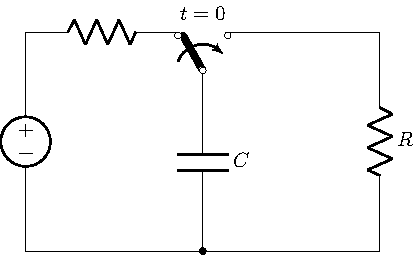
\includegraphics[height = 4cm, keepaspectratio = true]{rc_natural}
        \caption{RC circuit.}
        % \label{}
    \end{figure}
    By solving this differential equation, we can determine the natural response of a
    RC circuit.
    \begin{equation*}
        v(t) = v(0)\exp{\left( -\frac{t}{RC} \right)}
    \end{equation*}
    \begin{figure}[H]
        \centering
        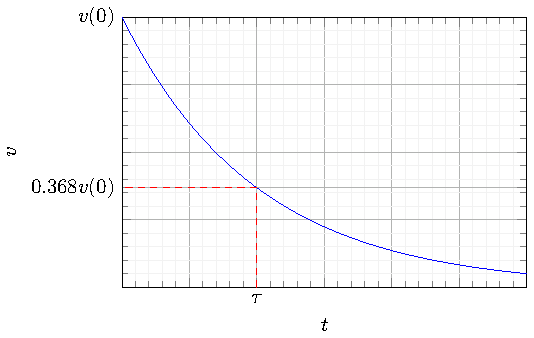
\includegraphics[height = 4cm, keepaspectratio = true]{rc_natural_plot}
        \caption{Natural response of a RC circuit.}
        % \label{}
    \end{figure}
\end{definition}
\begin{definition}[Time Constant]
    The time constant $\tau$ is a parameter for switching circuits. The time constant for a RC circuit is given by
    \begin{equation*}
        \tau = RC
    \end{equation*}
    The voltage at this time is equal to
    \begin{equation*}
        \e^{-1}v(0) \approx 0.368v(0)
    \end{equation*}
\end{definition}
\begin{definition}[RL Circuit Natural Response]
    For the circuit shown below, using mesh analysis gives the following relationship
    \begin{equation*}
        L \dv{i}{t} = -iR.
    \end{equation*}
    \begin{figure}[H]
        \centering
        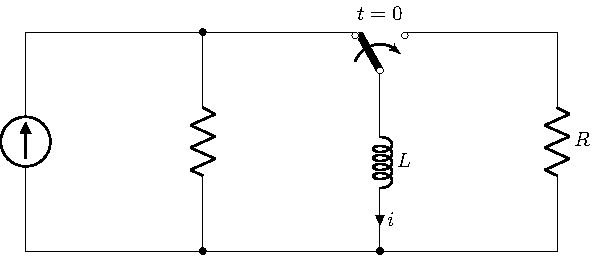
\includegraphics[height = 4cm, keepaspectratio = true]{rl_natural}
        \caption{RL circuit.}
        % \label{}
    \end{figure}
    By solving this differential equation, we can determine the natural response of a
    RL circuit.
    \begin{equation*}
        i(t) = i(0)\exp{\left( -\frac{t}{\frac{1}{R}L} \right)}
    \end{equation*}
    \begin{figure}[H]
        \centering
        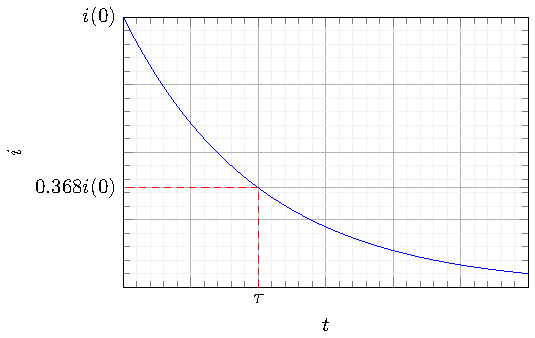
\includegraphics[height = 4cm, keepaspectratio = true]{rl_natural_plot}
        \caption{Natural response of a RL circuit.}
        % \label{}
    \end{figure}
\end{definition}
\begin{definition}[Time Constant]
    The time constant $\tau$ is a parameter for switching circuits. The time constant for a RL circuit is given by
    \begin{equation*}
        \tau = \frac{1}{R}L.
    \end{equation*}
    The current at this time is equal to
    \begin{equation*}
        \e^{-1}i(0) \approx 0.368i(0).
    \end{equation*}
\end{definition}
\subsection{Step Response}
\begin{definition}[RC Circuit Step Response]
    For the circuit shown below, using KCL at the top node gives the following relationship
    \begin{equation*}
        i_s = C\dv{v}{t} + \frac{v}{R}.
    \end{equation*}
    \begin{figure}[H]
        \centering
        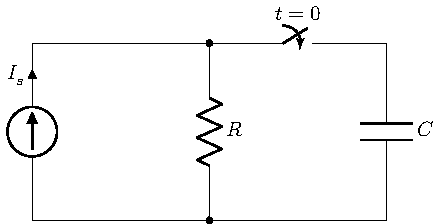
\includegraphics[height = 4cm, keepaspectratio = true]{rc_step}
        \caption{RC circuit.}
        % \label{}
    \end{figure}
    By solving this differential equation, we can determine the step response of a
    RC circuit.
    \begin{equation*}
        v(t) = I_sR + \left(V_0 - I_sR\right) \exp{\left( -\frac{t}{RC} \right)}
    \end{equation*}
    \begin{figure}[H]
        \centering
        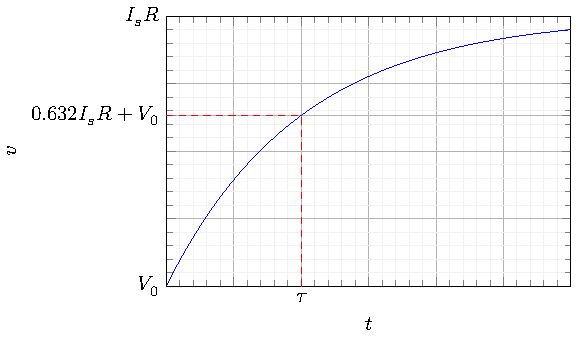
\includegraphics[height = 4cm, keepaspectratio = true]{rc_step_plot}
        \caption{Step response of a RC circuit.}
        % \label{}
    \end{figure}
    The voltage at $t = \tau$ is equal to
    \begin{align*}
        v(\tau) & = \left(1 - \e^{-1}\right)I_sR + V_0 \\
                & \approx 0.632I_sR + V_0.
    \end{align*}
\end{definition}
\begin{definition}[RL Circuit Step Response]
    For the circuit shown below, using mesh analysis gives the following relationship
    \begin{equation*}
        L\dv{i}{t} + iR = V_s.
    \end{equation*}
    \begin{figure}[H]
        \centering
        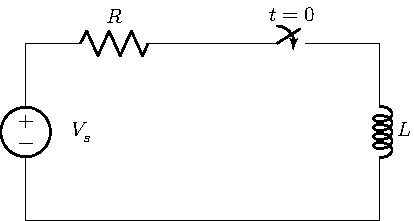
\includegraphics[height = 4cm, keepaspectratio = true]{rl_step}
        \caption{RL circuit.}
        % \label{}
    \end{figure}
    By solving this differential equation, we can determine the step response of a
    RL circuit.
    \begin{equation*}
        i(t) = \frac{V_s}{R} + \left(I_0 - \frac{V_s}{R}\right)\exp{\left( -\frac{t}{\frac{1}{R}L} \right)}
    \end{equation*}
    \begin{figure}[H]
        \centering
        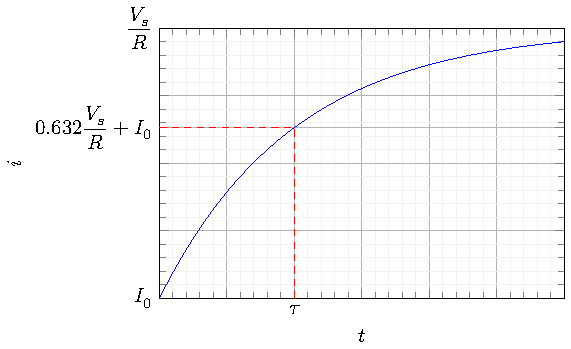
\includegraphics[height = 4cm, keepaspectratio = true]{rl_step_plot}
        \caption{Step response of a RL circuit.}
        % \label{}
    \end{figure}
    The current at $t = \tau$ is equal to
    \begin{align*}
        i(\tau) & = \left( 1 - \e^{-1} \right)\frac{V_s}{R} + I_0 \\
                & \approx 0.632\frac{V_s}{R} + I_0.
    \end{align*}
\end{definition}
\newpage
\section{Operational Amplifiers}
\begin{definition}[Amplifier]
    An amplifier is a device for increasing the power of a signal through an external energy source.
    In an electronic amplifier, the ``signal'' is usually a voltage or current.
\end{definition}
\begin{definition}[Gain]
    The gain $K$ of an amplifier, is the ratio of the output signal to the input signal.
    \begin{equation*}
        v_{out} = K v_{in}
    \end{equation*}
\end{definition}
\begin{definition}[Operational Amplifier]
    An operational amplifier (op amp) amplifies the voltage difference between its input terminals.
    Operational amplifiers require a power supply to amplify voltage.
    In an operational amplifier:
    \begin{enumerate}
        \item The output cannot exceed the power supply range.
        \item The inputs should remain within the power supply range.
    \end{enumerate}
    The output voltage has the following possibilities:
    \begin{enumerate}
        \item If $v_p - v_n > 0$, $v_{out} = V_{CC}$.
        \item If $v_p - v_n < 0$, $v_{out} = V_{EE}$.
        \item If $v_p - v_n = 0$, $v_{out} = 0$.
    \end{enumerate}
    \begin{figure}[H]
        \centering
        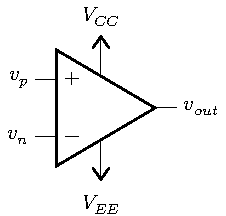
\includegraphics[height = 6cm, keepaspectratio = true]{operational_amplifier}
        \caption{Operational amplifier circuit symbol.}
        % \label{}
    \end{figure}
    \begin{description}
        \item[$v_p$:] non-inverting input
        \item[$v_n$:] inverting input
        \item[$V_{CC}$:] positive power supply
        \item[$V_{EE}$:] negative power supply
    \end{description}
\end{definition}
\subsection{Golden Rules for Op Amps}
\begin{enumerate}
    \item Infinite input impedance, therefore, zero input current.
    \item In a closed loop, the output drives the voltage difference at the inputs to zero.
\end{enumerate}
Note that the second rule only applies when the op amp has external negative feedback.
\subsection{Op Amp Analysis}
Using the golden rules above, the following circuits can be constructed.
\subsubsection{Inverting Amplifier}
\begin{equation*}
    v_{out} = -\frac{R_2}{R_1}v_{in}
\end{equation*}
\begin{figure}[H]
    \centering
    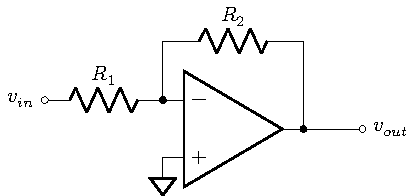
\includegraphics[width = 6cm, keepaspectratio = true]{inverting_amplifier}
    \caption{Inverting amplifier.}
\end{figure}
\subsubsection{Non-Inverting Amplifier}
\begin{equation*}
    v_{out} = \frac{R_1 + R_2}{R_1}v_{in}
\end{equation*}
\begin{figure}[H]
    \centering
    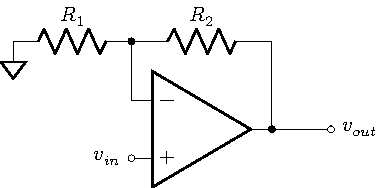
\includegraphics[width = 6cm, keepaspectratio = true]{non_inverting_amplifier}
    \caption{Non-inverting amplifier.}
\end{figure}
\subsubsection{Voltage Follower}
\begin{equation*}
    v_{out} = v_{in}
\end{equation*}
\begin{figure}[H]
    \centering
    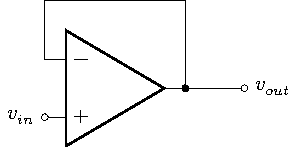
\includegraphics[width = 6cm, keepaspectratio = true]{voltage_follower}
    \caption{Voltage follower.}
\end{figure}
\subsubsection{Inverting Summing Amplifier}
\begin{equation*}
    v_{out} = -R_f \left( \frac{v_1}{R_1} + \frac{v_2}{R_2} + \cdots + \frac{v_n}{R_n} \right)
\end{equation*}
where $R_f$ is the feedback resistor.
\begin{figure}[H]
    \centering
    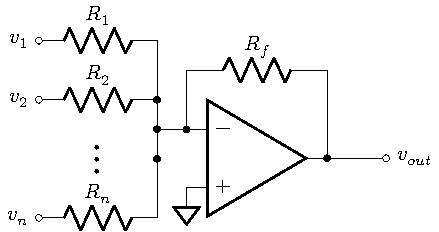
\includegraphics[width = 6cm, keepaspectratio = true]{inverting_summing_amplifier}
    \caption{Inverting summing amplifier.}
\end{figure}
\subsubsection{Difference Amplifier}
\begin{equation*}
    v_{out} = \frac{R_2}{R_1} \left( v_2 - v_1 \right)
\end{equation*}
where the ratio of $\displaystyle \frac{R_2}{R_1}$ must be equal on both legs.
\begin{figure}[H]
    \centering
    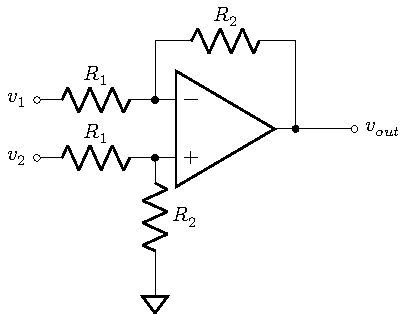
\includegraphics[width = 6cm, keepaspectratio = true]{difference_amplifier}
    \caption{Difference amplifier.}
\end{figure}
\subsection{Designing Op Amps}
When designing op amps, it is important to choose resistors in the $\qtyrange{1}{100}{\kilo\ohm}$
range, to prevent damaging the op amp, and to avoid excessive output currents.
\newpage
\section{Sinusoidal Signals}
\begin{definition}
    A sinusoidal signal is commonly referred to as Alternating Current or AC.
\end{definition}
\begin{figure}[H]
    \centering
    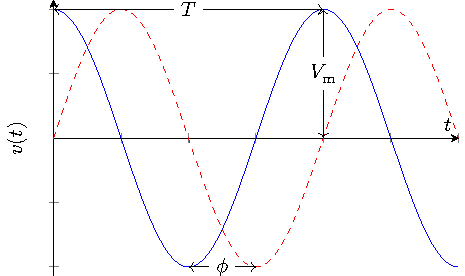
\includegraphics[height = 6cm, keepaspectratio = true]{sinusoidal_signal}
    \caption{Sinusoidal signals.}
\end{figure}
\subsection{Properties of Sinusoidal Signals}
These signals are described using cosine functions in the following form.
\begin{equation*}
    v(t) = V_{\mathrm{m}} \cos{\left( \omega t + \phi\si{\degree} \right)}
\end{equation*}
\subsubsection{Magnitude}
\begin{definition}
    The magnitude of a signal is the greatest distance from the line of oscillation, commonly zero,
    to the peak of the signal.
\end{definition}
\subsubsection{Angular Frequency}
\begin{definition}
    The angular frequency $\omega$ is measured in radians per second (\si{\radian\per\second}), and it allows
    us to compute the cosine function in radians.
\end{definition}
\subsubsection{Period and Frequency}
\begin{definition}[Period]
    The period of a signal $T$ is its cycle time in seconds (\si{\second}).
\end{definition}
\begin{definition}[Frequency]
    The frequency of a signal $f$ is the number of cycles per second, or
    the inverse of the period. The frequency is measured in Hertz (\si{\hertz}).
\end{definition}
The following equations relate the angular frequency, period and frequency together.
\begin{align*}
    f = \frac{1}{T} &  & T = \frac{2\pi}{\omega} &  & \omega = 2 \pi f
\end{align*}
\subsubsection{Phase}
\begin{definition}
    The phase $\phi$ of a signal is the position of a signal relative to a zero phase signal,
    measured in degrees (\si{\degree}). A \textbf{positive} phase corresponds to a ``leading''
    signal, and a \textbf{negative} phase corresponds to a ``lagging'' signal.
    The phase can be determined by calculating the difference in time $\tau$ between two signals.
    \begin{equation*}
        \phi = \frac{\tau}{T}
    \end{equation*}
\end{definition}
\subsection{Root Mean Square}
\begin{definition}
    Root mean square (rms) is a method of obtaining a useful average of a signal that is symmetric about
    the horizontal axis. It is defined as the square \textbf{root} of the \textbf{mean} value of the
    function \textbf{squared}.
    For a sine wave
    \begin{equation*}
        V_{\mathrm{rms}} = \frac{V_{\mathrm{m}}}{\sqrt{2}}
    \end{equation*}
    The units in rms quantities are also subscripted with rms, for example, rms voltage, $\si{\volt}_{\mathrm{rms}}$.
\end{definition}
\subsection{Power}
\begin{definition}
    In a resistive load, the power can be determined using the rms current and rms voltage.
    \begin{align*}
        p & = vi                                                                                         \\
        % p & = \sqrt{2}V_{\mathrm{rms}}\cos{\left( \omega t + \phi \right)}\sqrt{2}I_{\mathrm{rms}}\cos{\left( \omega t + \phi \right)} \\
        % p & = 2V_{\mathrm{rms}}I_{\mathrm{rms}}\cos^2{\left( \omega t + \phi \right)}                                                  \\
        p & = V_{\mathrm{rms}}I_{\mathrm{rms}}\bigl( 1 + \cos{\left( 2 \omega t + 2 \phi \right)} \bigr)
    \end{align*}
    The average power is given by
    \begin{equation*}
        P_{\mathrm{avg}} = V_{\mathrm{rms}}I_{\mathrm{rms}}
    \end{equation*}
\end{definition}
\subsection{Euler's Formula}
\begin{theorem}\label{theorem:eulers_formula}
    \begin{equation*}
        \e^{j\phi} = \cos{\left( \phi \right)} + j \sin{\left( \phi \right)}
    \end{equation*}
    where $j^2 = -1$ and $\phi$ is measured in radians.
\end{theorem}
\subsection{Phasors}
\begin{definition}
    To assist in AC analysis, we can express the magnitude and phase of a sinusoidal signal
    as a phasor.
\end{definition}
\subsection{Phasor Transforms}
\begin{definition}
    A sinusoidal signal can be converted to a phasor using the Phasor Transform
    \begin{align*}
        \symbf{V} & = \mathscr{P}\left\{ v(t) \right\}                                              \\
                  & = \mathscr{P}\bigl\{ V_{\mathrm{m}}\cos{\left( \omega t + \phi \right)} \bigr\} \\
                  & = V_{\mathrm{m}} \e^{j\phi}
    \end{align*}
    Here $\symbf{V}$ is the phase-domain representation of the
    time-domain signal $v(t)$.
    The magnitude and phase of a phasor can be used to represent a phasor in polar form
    \begin{equation*}
        \symbf{V} = V_{\mathrm{m}} \phase{\phi}
    \end{equation*}
\end{definition}
\subsection{Inverse Phasor Transforms}
\begin{definition}
    A phasor can be converted back to a sinusoidal signal using the Inverse Phasor Transform
    \begin{align*}
        v(t) & = \mathscr{P}^{-1}\left\{ \symbf{V} \right\}         \\
             & = \Re\left\{ \symbf{V} \e^{j\omega t} \right\}       \\
        %  & = \Re\left\{ V_{\mathrm{m}} \e^{j\phi} \e^{j\omega t} \right\}           \\
        %  & = V_{\mathrm{m}}\Re\left\{ \e^{j\left( \omega t + \phi \right)} \right\} \\
             & = V_{\mathrm{m}}\cos{\left( \omega t + \phi \right)}
    \end{align*}
\end{definition}
\subsection{Phasor Operations}
As phasors are quantities with a magnitude and angle, they can be represented as complex numbers.
Using \hyperref[theorem:eulers_formula]{Theorem \ref{theorem:eulers_formula}}, we can represent a phasor in rectangular form
\begin{equation*}
    \symbf{V} = V_{\mathrm{m}} \cos{\left( \phi \right)} + j V_{\mathrm{m}} \sin{\left( \phi \right)}
\end{equation*}
in polar form, the magnitude is given by
\begin{equation*}
    \norm{\symbf{V}} = V_{\mathrm{m}} = \sqrt{\Re\left\{ \symbf{V} \right\}^2 + \Im\left\{ \symbf{V} \right\}^2}
\end{equation*}
and the angle
\begin{equation*}
    \arg{\left( \symbf{V} \right)} = \phi = \arctan{\left( \frac{\Im\left\{ \symbf{V} \right\}}{\Re\left\{ \symbf{V} \right\}} \right)}
\end{equation*}
where $-\pi < \phi \leq \pi$.
\subsubsection{Addition with Phasors}
Phasors in rectangular form can be added using their real and imaginary parts.
\begin{align*}
    \symbf{A} + \symbf{B} & = \Re\left\{ \symbf{A} + \symbf{B} \right\} + \Im\left\{ \symbf{A} + \symbf{B} \right\}                                                                                                                      \\
                          & = \bigl( A_{\mathrm{m}}\cos{\left( \phi_1 \right)} + B_{\mathrm{m}}\cos{\left( \phi_2 \right)} \bigr) + j\bigl( A_{\mathrm{m}}\sin{\left( \phi_1 \right)} + B_{\mathrm{m}}\sin{\left( \phi_2 \right)} \bigr)
\end{align*}
\subsubsection{Multiplication with Phasors}
Phasors in polar form can be multiplied using their magnitudes and phases.
\begin{align*}
    \symbf{A} \symbf{B} & = \norm{\symbf{A}} \norm{\symbf{B}} \phase{\arg{\left( \symbf{A} \right)} + \arg{\left( \symbf{B} \right)}} \\
                        & = A_{\mathrm{m}} B_{\mathrm{m}} \phase{\phi_1 + \phi_2}
\end{align*}
\subsection{Circuit Analysis}
\begin{theorem}[Phasor Relationship for Resistors]
    \begin{equation*}
        \symbf{V} = \symbf{I} R
    \end{equation*}
\end{theorem}
\begin{proof}
    Using a sinusoidal voltage
    \begin{equation*}
        v = V_{\mathrm{m}}\cos{\left( \omega t + \phi \right)}
    \end{equation*}
    Ohm's Law gives:
    \begin{align*}
        i & = \frac{v}{R}                                                   \\
          & = \frac{V_{\mathrm{m}}}{R} \cos{\left( \omega t + \phi \right)}
    \end{align*}
    Taking the Phasor Transform gives
    \begin{align*}
        \mathscr{P}\left\{ v \right\}                                                  & = \mathscr{P}\left\{ iR \right\}                                                              \\
        \mathscr{P}\left\{ V_{\mathrm{m}}\cos{\left( \omega t + \phi \right)} \right\} & = \mathscr{P}\left\{ \frac{V_{\mathrm{m}}}{R} \cos{\left( \omega t + \phi \right)} \right\} R \\
        \symbf{V}                                                                      & = \symbf{I} R
    \end{align*}
\end{proof}
\begin{theorem}[Phasor Relationship for Inductors]
    \begin{equation*}
        \symbf{V} = j\omega L\symbf{I}
    \end{equation*}
\end{theorem}
\begin{proof}
    Using a sinusoidal current
    \begin{equation*}
        i = I_{\mathrm{m}}\cos{\left( \omega t + \phi \right)}
    \end{equation*}
    the voltage drop across an inductor is given by:
    \begin{align*}
        v & = L \dv{i}{t}                                                                      \\
          & = -\omega L I_{\mathrm{m}} \sin{\left( \omega t + \phi \right)}                    \\
          & = -\omega L I_{\mathrm{m}} \cos{\left( \omega t + \phi - \SI{90}{\degree} \right)}
    \end{align*}
    taking the Phasor Transform gives
    \begin{align*}
        \mathscr{P}\left\{ v \right\} & = \mathscr{P}\left\{ L \dv{i}{t} \right\}                                                                      \\
        \symbf{V}                     & = \mathscr{P}\left\{ -\omega L I_{\mathrm{m}} \cos{\left( \omega t + \phi - \SI{90}{\degree} \right)} \right\} \\
        \symbf{V}                     & = -\omega L I_{\mathrm{m}} \e^{j\left( \phi - \SI{90}{\degree} \right)}                                        \\
        \symbf{V}                     & = -\omega L I_{\mathrm{m}} \e^{j \phi} \e^{-j\SI{90}{\degree}}                                                 \\
        \symbf{V}                     & = j\omega L I_{\mathrm{m}} \e^{j \phi}                                                                         \\
        \symbf{V}                     & = j\omega L \symbf{I}
    \end{align*}
\end{proof}
\begin{theorem}[Phasor Relationship for Capacitors]
    \begin{equation*}
        \symbf{V} = \frac{1}{j\omega C}\symbf{I}
    \end{equation*}
\end{theorem}
\begin{proof}
    Using a sinusoidal voltage
    \begin{equation*}
        v = V_{\mathrm{m}}\cos{\left( \omega t + \phi \right)}
    \end{equation*}
    the voltage-current relationship across a capacitor is given by:
    \begin{align*}
        i & = C \dv{v}{t}                                                                      \\
          & = -\omega C V_{\mathrm{m}} \sin{\left( \omega t + \phi \right)}                    \\
          & = -\omega C V_{\mathrm{m}} \cos{\left( \omega t + \phi - \SI{90}{\degree} \right)}
    \end{align*}
    taking the Phasor Transform gives
    \begin{align*}
        \mathscr{P}\left\{ i \right\} & = \mathscr{P}\left\{ C \dv{v}{t} \right\}                                                                      \\
        \symbf{I}                     & = \mathscr{P}\left\{ -\omega C V_{\mathrm{m}} \cos{\left( \omega t + \phi - \SI{90}{\degree} \right)} \right\} \\
        \symbf{I}                     & = -\omega C V_{\mathrm{m}} \e^{j\left( \phi - \SI{90}{\degree} \right)}                                        \\
        \symbf{I}                     & = -\omega C V_{\mathrm{m}} \e^{j \phi} \e^{-j\SI{90}{\degree}}                                                 \\
        \symbf{I}                     & = j\omega C V_{\mathrm{m}} \e^{j \phi}                                                                         \\
        \symbf{I}                     & = j\omega C \symbf{V}                                                                                          \\
        \symbf{V}                     & = \frac{1}{j\omega C} \symbf{I}
    \end{align*}
\end{proof}
\subsection{Impedance}
\begin{definition}
    The impedance $\symbf{Z}$ of an element, measured in Ohms (\si{\ohm}), is its opposition to alternating current.
    Impedance is represented as the sum of a real resistance $R$ and imaginary reactance $X$.
    \begin{equation*}
        \symbf{Z} = R + jX
    \end{equation*}
    Impedance captures the magnitude and phase change associated with a circuit element.
\end{definition}
\begin{theorem}[Impedance of Resistors]
    \begin{equation*}
        \symbf{Z} = R
    \end{equation*}
\end{theorem}
\begin{theorem}[Impedance of Inductors]
    \begin{equation*}
        \symbf{Z} = j\omega L
    \end{equation*}
\end{theorem}
\begin{theorem}[Impedance of Capacitors]
    \begin{equation*}
        \symbf{Z} = \frac{1}{j\omega C}
    \end{equation*}
\end{theorem}
\subsection{Impedances in Circuits}
\begin{theorem}
    Impedances behave similarly to resistances in series and parallel.
\end{theorem}
\newpage
\section{Frequency Response}
Frequency response is a measure of the magnitude and phase of a system as a function of (angular) frequency $\omega$.
\subsection{Circuit Analysis with AC Circuits}
\begin{theorem}
    Any DC analysis technique can be used with AC circuits, as long as
    resistive elements are represented using complex impedances.
\end{theorem}
\subsection{Transfer Function}
\begin{definition}
    The transfer function of a system is given by
    \begin{equation*}
        \symbf{H}(\omega) = \frac{\symbf{Y}(\omega)}{\symbf{X}(\omega)}
    \end{equation*}
    where $\symbf{Y}$ is the output and $\symbf{X}$ is the input of a system.
\end{definition}
\begin{definition}[Linear Gain]
    The magnitude of the transfer function $\norm{\symbf{H}}$ measures the linear gain of a system.
\end{definition}
\begin{definition}[Gain in \si{\decibel}]
    The gain of a system is often represented in \si{\decibel} using the following formula
    \begin{equation*}
        \mathrm{gain} = 20 \log_{10}{\norm{\symbf{H}}}
    \end{equation*}
\end{definition}
\begin{definition}[Phase Shift]
    The phase of the transfer function $\arg{\left( \symbf{H} \right)}$ measures the phase shift of a system.
\end{definition}
\subsection{Bode Plots}
A Bode plot is a graph of the frequency response of a system.
In this plot, the frequency (in \si{\hertz}) is plotted on the horizontal axis using a logarithmic scale.
\begin{definition}[\SI{3}{\decibel} Point]
    The frequency $f$ at which the transfer function equals
    \begin{equation*}
        \symbf{H}(2\pi f) = \frac{1}{\sqrt{2}}\phase{\SI{-45}{\degree}}
    \end{equation*}
    is known as the break frequency, corner frequency,
    \SI{3}{\decibel} frequency, or half power point.

    This is because the gain at this point is equal to $\SI{0.707} \approx \SI{-3.01}{\decibel}$,
    and the angle \SI{-45}{\degree} is the halfway point between \SI{0}{\degree} and \SI{-90}{\degree}.
\end{definition}
\begin{figure}[H]
    \centering
    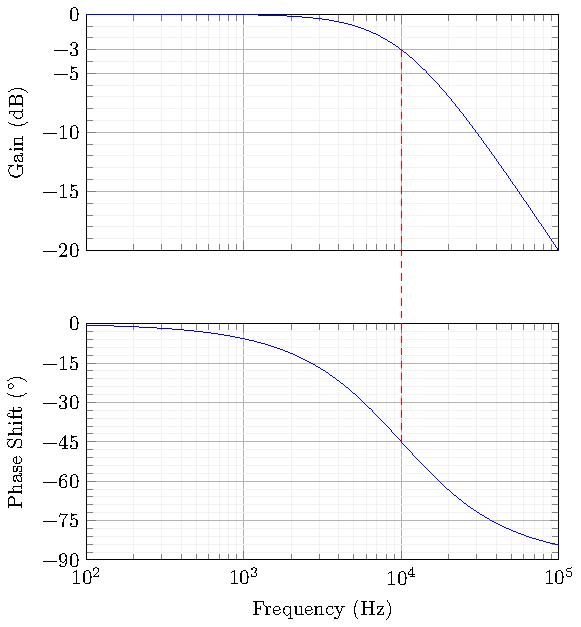
\includegraphics[width = \linewidth, keepaspectratio = true]{bode_plot}
    \caption{Bode plot of gain and phase shift.}
\end{figure}
\newpage
\section{Filters and Rectifiers}
\begin{definition}[Filters]
    A filter is designed to allow certain ranges of frequencies to pass,
    while other ranges of frequencies are stopped.
\end{definition}
\begin{definition}[Cut-off Frequncy]
    The cut-off (angular) frequency $\omega_c$ for a filter is given by
    \begin{equation*}
        \omega_c = \frac{1}{RC}
    \end{equation*}
\end{definition}
\subsection{Common Filters}
\begin{figure}[H]
    \centering
    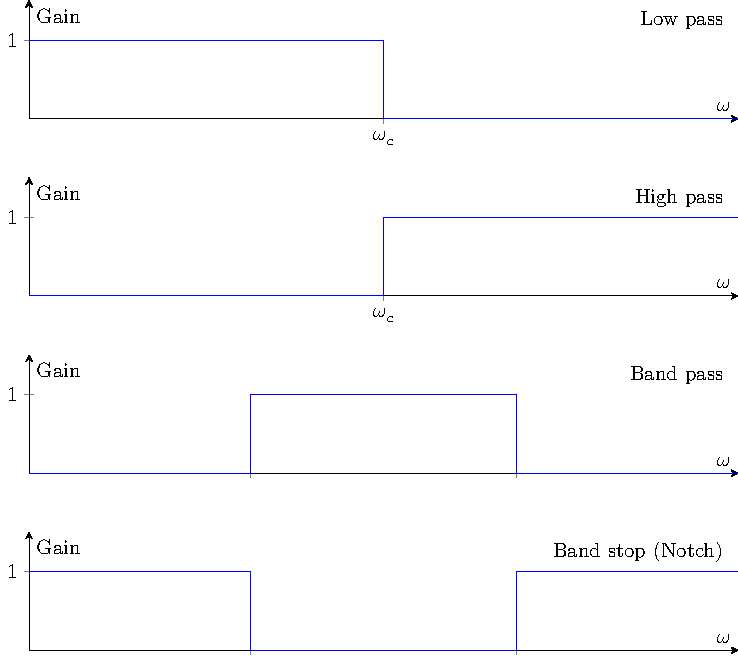
\includegraphics[height = 9cm, keepaspectratio = true]{filters}
    \caption{Different types of filters.}
\end{figure}
\subsection{Passive Filters}
Passive filters are circuits containing only passive elements
(such as resistors, capacitors and inductors),
which filter unwanted parts of a signal.
Passive filters are affected by loading, such that a varied load will
affect the cut-off frequency.
\subsubsection{Low Pass Filter}
The following low pass filter has the following transfer function.
\begin{equation*}
    \symbf{H}(\omega) = \frac{\omega_c}{j\omega + \omega_c}
\end{equation*}
where $\displaystyle \omega_c = \frac{1}{RC}$.
\begin{figure}[H]
    \centering
    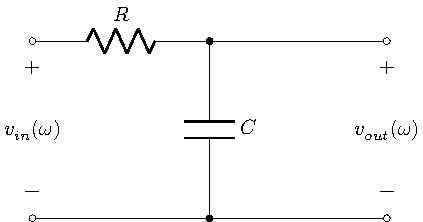
\includegraphics[width = 8cm, keepaspectratio = true]{passive_low_pass_filter}
    \caption{Passive low pass filter.}
\end{figure}
\subsubsection{High Pass Filter}
The following high pass filter has the following transfer function.
\begin{equation*}
    \symbf{H}(\omega) = \frac{j\omega}{j\omega + \omega_c}
\end{equation*}
where $\displaystyle \omega_c = \frac{1}{RC}$.
\begin{figure}[H]
    \centering
    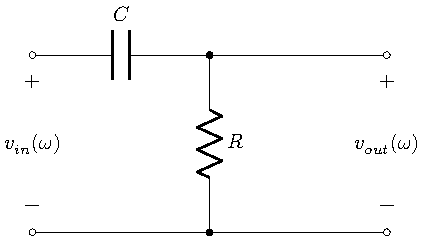
\includegraphics[width = 8cm, keepaspectratio = true]{passive_high_pass_filter}
    \caption{Passive high pass filter.}
\end{figure}
\subsection{Active Filters}
Active filters are circuits containing active elements (such as op amps),
which filter unwanted parts of a signal.
Active filters are not affected by loading, such that a varied load will
not affect the cut-off frequency.

For the following active filters, the gain component is given by
\begin{equation*}
    \mathrm{gain} = -\frac{R_2}{R_1}
\end{equation*}
\subsubsection{Low Pass Filter}
The following low pass filter has the following transfer function.
\begin{equation*}
    \symbf{H}(\omega) = -\frac{R_2}{R_1}\frac{\omega_c}{j\omega + \omega_c}
\end{equation*}
where $\displaystyle \omega_c = \frac{1}{R_2C}$.
\begin{figure}[H]
    \centering
    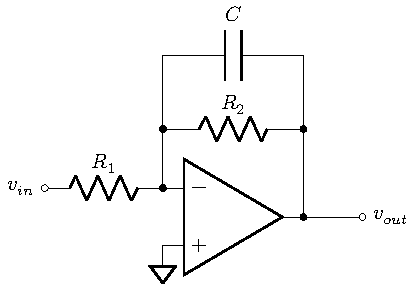
\includegraphics[width = 8cm, keepaspectratio = true]{active_low_pass_filter}
    \caption{Active low pass filter.}
\end{figure}
\subsubsection{High Pass Filter}
The following high pass filter has the following transfer function.
\begin{equation*}
    \symbf{H}(\omega) = -\frac{R_2}{R_1}\frac{j\omega}{j\omega + \omega_c}
\end{equation*}
where $\displaystyle \omega_c = \frac{1}{R_1C}$.
\begin{figure}[H]
    \centering
    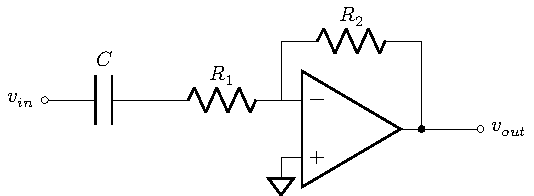
\includegraphics[width = 8cm, keepaspectratio = true]{active_high_pass_filter}
    \caption{Active high pass filter.}
\end{figure}
\subsection{Rectifiers}
\begin{definition}[Plugpack]
    An AC plugpack steps the mains AC voltage (\SI{240}{\volt} RMS) down to a safe AC voltage level.
\end{definition}
\begin{definition}[Rectifier]
    A rectifier is designed to convert AC signals to DC.
\end{definition}
By using a diode, a rectifier only allows current to pass when an AC
voltage is positive.
\begin{figure}[H]
    \centering
    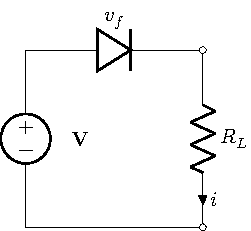
\includegraphics[height = 4cm, keepaspectratio = true]{half_wave_rectifier_without_capacitor}
    \caption{Half-wave rectifier circuit without capacitor.}
\end{figure}
\begin{figure}[H]
    \centering
    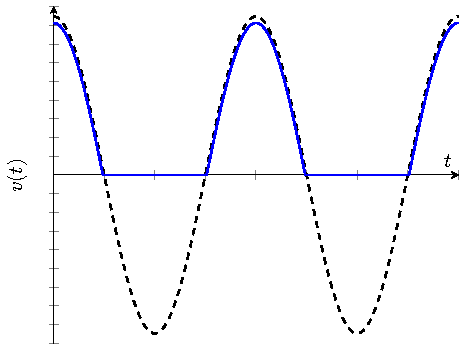
\includegraphics[width = 8cm, keepaspectratio = true]{half_wave_rectifier_without_capacitor_plot}
    \caption{Half-wave rectified signal.}
\end{figure}
\begin{definition}[Ripple]
    Ripple is the residual variation of the DC voltage after rectification.
    In the circuit shown above, a capacitor can be used to smooth ripples.

    Ripple can be calculated using the following assumptions:
    \begin{enumerate}
        \item The capacitor instantly charges when the diode is forward biased.
        \item The capacitor discharges with a constant current.
    \end{enumerate}
    The VI relationship for a capacitor gives the following formula for ripple
    \begin{equation*}
        \Delta v = \frac{i}{C} \Delta t
    \end{equation*}
    where $f$ is the frequency of the voltage source.
\end{definition}
\subsubsection{Half-wave Rectifier}
\begin{figure}[H]
    \centering
    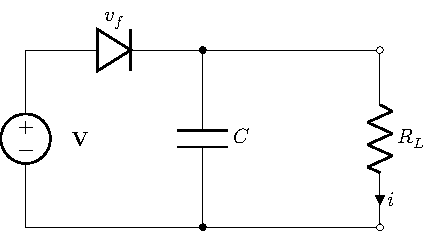
\includegraphics[width = 8cm, keepaspectratio = true]{half_wave_rectifier}
    \caption{Half-wave rectifier circuit.}
\end{figure}
\begin{figure}[H]
    \centering
    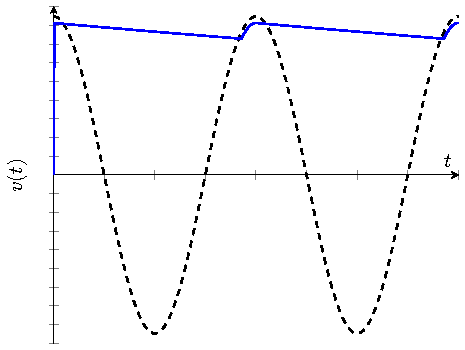
\includegraphics[width = 8cm, keepaspectratio = true]{half_wave_rectifier_plot}
    \caption{Half-wave rectified signal.}
\end{figure}
\begin{itemize}
    \item The diode conducts on the positive half cycle
    \item The output loses the forward voltage of one diode
\end{itemize}
The ripple in a half-wave rectifier is calculated using
\begin{equation*}
    \Delta v = \frac{i}{fC}
\end{equation*}
\subsubsection{Full-wave Rectifier}
\begin{figure}[H]
    \centering
    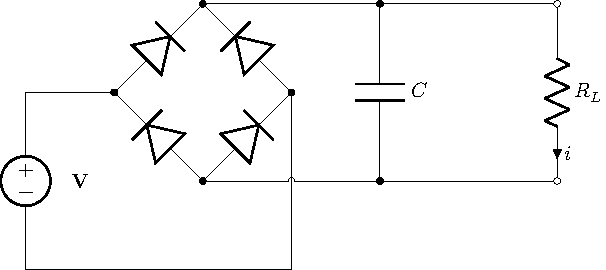
\includegraphics[width = 8cm, keepaspectratio = true]{full_wave_rectifier}
    \caption{Half-wave rectifier circuit.}
\end{figure}
\begin{figure}[H]
    \centering
    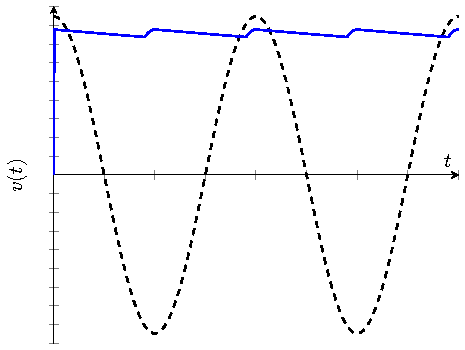
\includegraphics[width = 8cm, keepaspectratio = true]{full_wave_rectifier_plot}
    \caption{Full-wave rectified signal.}
\end{figure}
\begin{itemize}
    \item Two diodes conduct every half cycle
    \item The output loses the forward voltage of two diodes
\end{itemize}
The ripple in a full-wave rectifier is calculated using
\begin{equation*}
    \Delta v = \frac{i}{2fC}
\end{equation*}
\subsubsection{Dual half-wave Rectifier}
\begin{figure}[H]
    \centering
    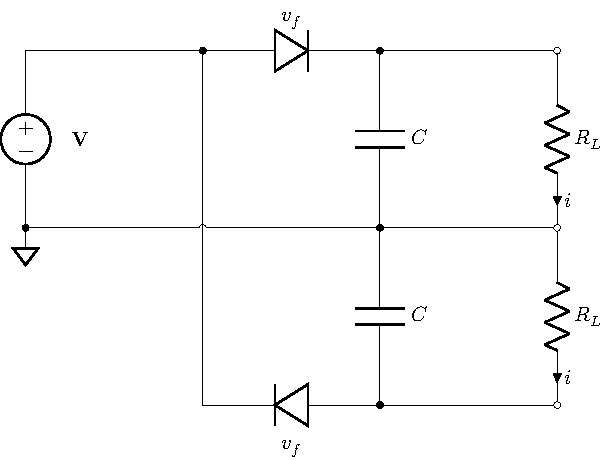
\includegraphics[width = 8cm, keepaspectratio = true]{dual_half_wave_rectifier}
    \caption{Dual half-wave rectifier circuit.}
\end{figure}
\begin{figure}[H]
    \centering
    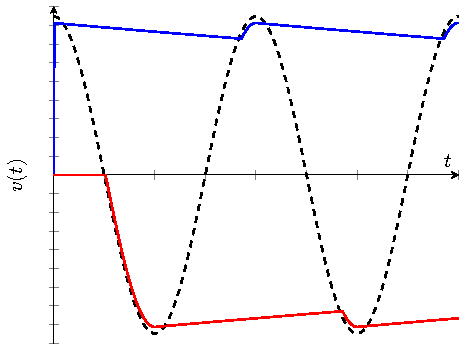
\includegraphics[width = 8cm, keepaspectratio = true]{dual_half_wave_rectifier_plot}
    \caption{Dual half-wave rectified signal.}
\end{figure}
\begin{itemize}
    \item The diodes conducts on both cycles
    \item The output loses the forward voltage of one diode
    \item Useful for powering op amps
\end{itemize}
The ripple in a dual half-wave rectifier is calculated using
\begin{equation*}
    \Delta v = \frac{i}{fC}
\end{equation*}
\newpage
\section{Zener Diodes and Voltage Regulators}
\subsection{Zener Diodes}
A Zener diode is similar to a regular diode, but it has a specific
reverse breakdown voltage. The reverse breakdown voltage is commonly \SI{5}{\volt}.
\begin{figure}[H]
    \centering
    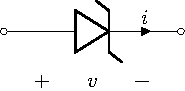
\includegraphics[height = 3cm, keepaspectratio = true]{zener_diode}
    \caption{Zener diode circuit diagram.}
\end{figure}
The ideal VI characteristic for a Zener diode is shown below.
\begin{figure}[H]
    \centering
    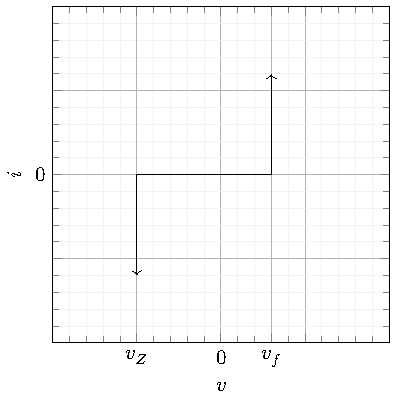
\includegraphics[height = 5cm, keepaspectratio = true]{vi_characteristic_zener_diode}
    \caption{VI characteristic for an ideal Zener diode.}
\end{figure}
\subsection{Voltage Regulators}
Most circuits require a clean DC power supply to operate.
A voltage regulator ensures that a DC power supply behaves like an ideal voltage source.
\subsection{Shunt Regulators}
\begin{definition}[Shunt Regulator]
    A shunt regulator regulates the output voltage by shunting excess current away from the load.
\end{definition}
A Zener diode can be used as a shunt regulator to drop voltages to the reverse bias voltage of the diode.
\begin{remark}
    When designing a Zener voltage regulator, the following should be taken into account:
    \begin{itemize}
        \item Power dissipation particularly when dropping large voltages.
        \item Large series resistances reduces power dissipation but also reduces the regulated current.
        \item A Zener voltage regulator always draws power from the source, regardless of the load.
        \item The load has an effect on the regulator.
    \end{itemize}
\end{remark}
\begin{figure}[H]
    \centering
    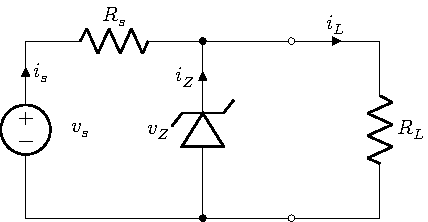
\includegraphics[height = 4cm, keepaspectratio = true]{zener_regulator}
    \caption{Zener diode regulator.}
\end{figure}
\begin{theorem}[Maximum Load Current.]
    Given a source voltage range $v_s$ and source resistance $R_s$, the maximum current an ideal
    Zener diode can regulate is given by
    \begin{equation*}
        i_L < \frac{v_s - v_Z}{R_s}
    \end{equation*}
    where the largest value in $v_s$ is chosen.
\end{theorem}
\begin{theorem}[Maximum Source Resistance.]
    Given a source voltage range $v_s$ and load current range $i_L$, the maximum source resistance required
    to regulate the output voltage is given by
    \begin{equation*}
        R_s < \frac{v_s - v_Z}{i_L}
    \end{equation*}
    where the smallest value in $v_s$ is chosen, and the largest value in $i_L$ is chosen.
\end{theorem}
\begin{proof}
    Using KCL gives
    \begin{align*}
        i_s - i_Z & = i_L        \\
        i_Z       & = i_s - i_L.
    \end{align*}
    For a Zener diode to operate at its reverse breakdown voltage, the Zener current
    must be nonzero. This gives
    \begin{equation*}
        0 < \frac{v_s - v_Z}{R_s} - i_L
    \end{equation*}
    We must now consider the worst case scenario, namely, when
    $\displaystyle \frac{v_s - v_Z}{R_s}$ is minimised, and when $i_L$ is maximised.

    Hence the maximum load current is when $v_s$ is maximal.

    And the maximum source resistance is when $v_s$ is minimal, and $i_L$ is maximal.
\end{proof}
\subsection{Series Regulators}
\begin{definition}[Series Regulator]
    Series regulators regulate the output voltage by limiting the load current by varying the series element.
\end{definition}
\subsubsection{Series Linear Regulators}
LM-series integrated circuits (IC) are a three-terminal linear regulator that regulate fixed voltages of \SI{0.5}{\volt} to \SI{24}{\volt}.
They require an input voltage at least \SI{2}{\volt} greater than the regulated output voltage.
An LM-series regulator circuit is shown below.
\begin{figure}[H]
    \centering
    \includegraphics[height = 4cm, keepaspectratio = true]{series_linear_regulator}
    \caption{Series Linear Regulator using an LM-series IC.}
\end{figure}
\emph{Note that the capacitors remain the same for any output voltage.}

The naming convention is as follows,
\begin{enumerate}
    \item LM78XX regulates a positive voltage XX\si{\volt}.
    \item LM79XX regulates a negative voltage -XX\si{\volt}.
\end{enumerate}
The power dissipation can be calculated by assuming 0 ground current.
\subsubsection{Power Supply Design}
A rectifier and regulator circuit can be combined to create a power supply from an AC voltage plugpack.
\begin{figure}[H]
    \centering
    \includegraphics[height = 4cm, keepaspectratio = true]{power_supply}
    \caption{AC to DC power supply circuit.}
\end{figure}
A dual half-wave rectifier can be used to supply positive and negative voltage.
\begin{figure}[H]
    \centering
    \includegraphics[width = \linewidth, keepaspectratio = true]{dual_power_supply}
    \caption{AC to DC dual power supply circuit.}
\end{figure}
The maximum ripple for these circuits is shown below.
\begin{align*}
    \max{\Delta v}                                  & = \max{v_{in}} - v_f - \left( 2 + v_{out} \right) \\
    \therefore\: \Delta v                           & > \frac{i}{fC}                                    \\
    \max{v_{in}} - v_f - \left( 2 + v_{out} \right) & > \frac{i}{fC}
\end{align*}
\subsubsection{Series Op Amp Regulators}
Op amps can be utilised stabilise the output from a regulator.
The op amp is powered by the source voltage and the series resistance is chosen to minimise the current to the Zener diode.
\begin{figure}[H]
    \centering
    \includegraphics[height = 8cm, keepaspectratio = true]{series_op_amp_regulator}
    \caption{Series op amp regulator circuit.}
\end{figure}
In the circuit above, $i_Z + i_S = 0$.

The power dissipated by the circuit can be determined by finding the power produced at the voltage source
which is given by
\begin{equation*}
    p = v_{in} \left( i_L - i_Z \right).
\end{equation*}
\end{document}